\section{Outline}
This thesis is structured into seven chapters.
\newline \\Chapter 1 narrates the background motivation, explains the current Norwegian healthcare influenza-related systems, and introduces the objectives for this thesis.
\newline \\Chapter 2 describes related works of what others have found useful as tools and other proven effective measurements.
\newline \\Chapter 3 marks out in detail the datasets used by this project, describes and give an explanation of relevance, challenges, limitation, and rewards.
\newline \\Chapter 4 outlines the implementation and graphical results of the datasets used in chapter 3.
\newline \\Chapter 5 shows the overall results.
\newline \\Chapter 6 discusses the results, project management, encountered constraints, ethical concerns and future work.
\newline \\Chapter 7 concludes this thesis.


\newpage


\section{Background}
Influenza is an exceedingly contagious viral infection which gives high fever, general pain, and respiratory symptoms\cite{fhi_sykdommer}. An estimated five to ten percent of the population becomes infected during the yearly influenza season, which is generally in the winter. The virus is especially dangerous to the elderly and to pregnant people from the second-trimester. Annually between the months of December and April people of the northern hemisphere are struck by influenza epidemics. Since this is a seasonal occurrence mitigation or even elimination of the effects are a priority and thus observation and research are initiated. From a historical perspective, it is known that influenza can have overwhelming destructive consequences if left unreservedly to ravage the population. The last three larger pandemics were the Asian flu of 1957, the flu of 1968 which originated in Hong Kong and the H1N1 (swine flu) virus of 2009, which respectively claimed the lives of 1.1 million, 1-4 million and 284500 people \cite{world2005ten}. The World Health Organization (WHO) estimates an annual global infection of humans to be a rate of 5-15\% \cite{who2017}, this causes 300.000 to 650.000 deaths per year\cite{iuliano2017estimates}, and about 1700 of these are Norwegians\cite{niph}. The virus mutates often which proves immunization by a vaccine to be a seasonal effort. Infection happens via droplets in the air inhaled, and even a small exposure expands to an all-out blitz which the immune system is forced to engage.

Diseases travel with humans as they commute or travel long distances and thus spread\cite{poletto2013human}\cite{wibisono2008non}. The gravity and influence of an infectious disease can have is also strongly correlated to social\cite{yang2017characterizing} and environmental\cite{robertson2017towards} circumstances. The intricate and fluctuating spread of contagious diseases within a complex and mobile human domain means that a static and a uniform approach is sub-optimal because the real grasp of the structure is a more changing operation with its own convoluted variety of variables \cite{spatiotemp_urban_sys}\cite{enduri2018dynamics}.

One of the fundamental requirements for efficient control of urban outbreaks is to maintain situational awareness of the extent, impact, and potential of ongoing outbreaks. To accomplish this, a series of clinical indicator-based surveillance systems monitor patient-general practitioner interaction, as well as laboratory-based analysis and intensive care unit (ICU) surveillance. 



The power to obtain enough information to detect possible trends of influenza seasons depends on successful integration between a multitude of different participants. Automatic extraction and processing of data is paramount for efficient analysis and gives a solid basis for an autonomous pathological detection system. Scalability is important in merging new relevant datasets as they become available in an ever-growing societal infrastructure. This thesis proposes a technology that would become an influential part of a bigger foundation intertwined with a robust knowledgeable and organizational means to mobilize assets in order to respond to possible outbreaks as or even before they start. Such a system requires as many feasible input channels from different urban systems and resources as possible in order to become reliable.


\newpage


\section{Influenza surveillance}
The current surveillance systems are heavily based on clinical indicators, and it is of interest to establish new mechanisms that make use of other indicators. Establishing surveillance systems based on societal indicators allow for detection of non-clinical factors that indicate the presence of influenza in society. Directly monitoring behaviour at the societal level may also provide the ability to detect emerging behaviour and pattern deviations that indicate the presence of influenza at an earlier stage than what can be accomplished through patient-doctor interaction.\\
The management of seasonal influenza outbreaks is handled by public health officials and epidemiologists with the use of the national surveillance system provided by the Norwegian Institute of Public Health (NIPH)\cite{niph}.
  
\begin{table}[!htb]
\begin{tabular}{ | m{9em} | m{10.4cm}| }
 \hline
 \textbf{System} & \textbf{Function} \\ [0.5ex] 
 \hline
 NorSySS & Indicator-based surveillance of influenza-like illness in primary health care \\ 
  \hline
 Hospital (all ward) surveillance  & Laboratory-based surveillance of hospitalised influenza cases \\[1ex]
  \hline
 ICU surveillance & ICU treated flu patients. Data collected by the Norwegian Intensive Care Registry (pilot project since 2016/17) \\
  \hline
 Virological-surveillance & (1) Submission of data and samples from Norwegian laboratories testing for influenza.
(2) Sentinel system, GP-based virological surveillance. \\[1ex]
  \hline
 Norwegian mortality monitoring system (NorMOMO) & Surveillance of weekly all-cause excess mortality. \\[1ex]
 \hline
 Seroepidemiological analysis & Annual survey of flu immunity in the population. \\ [1ex] 
 \hline
\end{tabular}
\caption{The Norwegian surveillance system for influenza}
 \label{table:1}
\end{table}

The Norwegian Syndromic Surveillance System (NorSySS) collects influenza-like illnesses (ILI) from general practitioners (GPs)\cite{NorSySS}, figure \ref{fig:norsyss} shows a diagram of their process. The current NorSySS system relies upon reports of influenza-like illness from general practitioners (GPs).  These subsystems compose part of the Norwegian influenza surveillance system and provide data with high reliability, but low timeliness. Typically the delay is over a week because it relies on clinical reports and laboratory endeavours, and leaves few ways to assess the societal impact of ongoing outbreaks.\\ Measuring societal indicators based on the spatiotemporal components inherent in these data sources makes it possible to draw upon spatial epidemiological traditions to link societal behaviour to outbreaks of seasonal influenza with a significantly higher temporal resolution than found in current flu monitoring systems. The goal of this thesis is to determine whether a monitoring system of urban real-time data could do the same with less delay.

\begin{figure}[!htb]
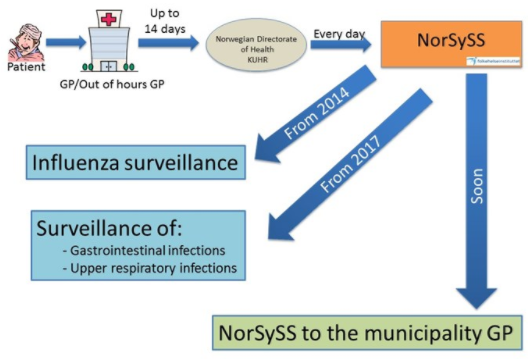
\includegraphics[width=3.5cm]{NorSySS_diagram}
\centering
\caption{NIPH, 2017}
\label{fig:norsyss}
\end{figure}

\newpage


\section{Spatiotemporal information from urban systems}
In the novel study of "Detecting flu outbreaks based on spatiotemporal information from an urban system", which is the base idea for this thesis, Grottenberg et al. \cite{spatiotemp_urban_sys} outlines a design for a system for surveillance of flu outbreaks. Emphasis on the belief that real-time data flows could prove useful in both understanding social functions during disasters and crisis as well as give "actionable intelligence for use in influenza management efforts.". The goal would be to extend the already implemented infrastructure with an approach to monitor human behaviour in trends throughout the influenza activity in hope for discrepancies detected through spatial analysis on important measurements. The borrowed figure \ref{fig:grottenberg} from his article sums up what this thesis hopes to accomplish, namely to find a correlation between different datasets and the datasets from the Norwegian public health institution (NIPH), this interference of public behaviour would become visible in essential criterion.


\begin{figure}[!htb]
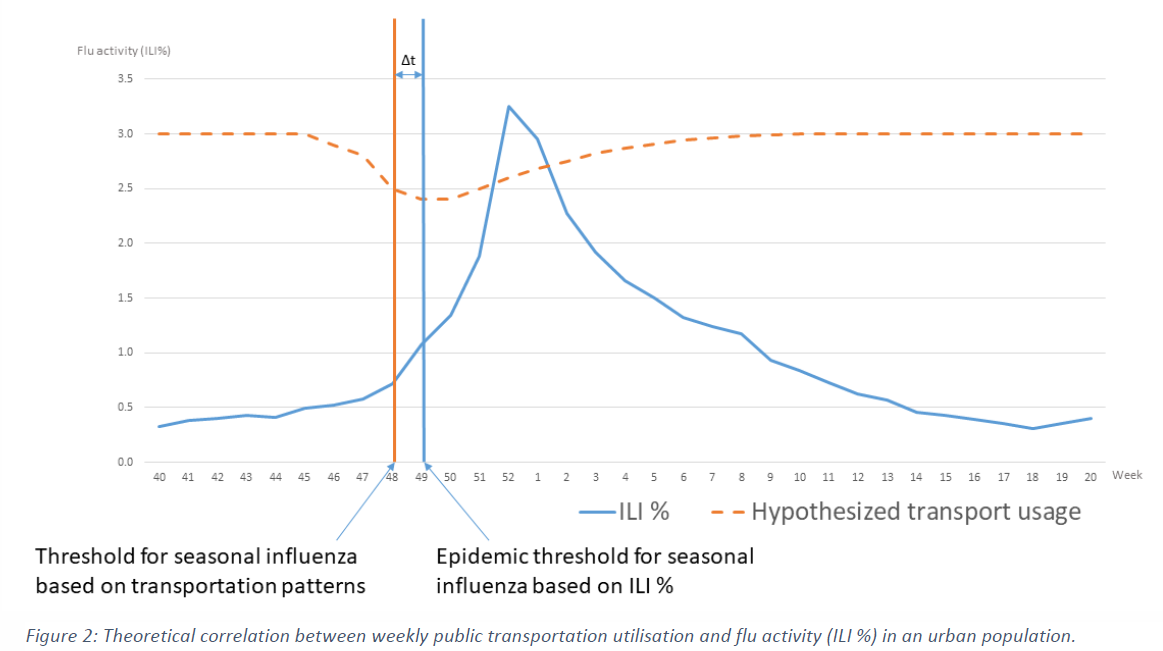
\includegraphics[width=13.5cm]{grottenberg}
\centering
\caption{Figure from Grottenberg et al. \cite{spatiotemp_urban_sys}}
\label{fig:grottenberg}
\end{figure}

\newpage


\section{Objectives}
This thesis examines the viability of investigating, collecting and analysing relevant urban true-time data for a self-sufficient influenza seasonal recognition system.\\
The main suggestion of this thesis is as influenza develops it reveals subtle patterns in societal behaviours that is detectable through a variety of mediums, e.g urban datasets from sewage, public transportation, medicinal purchases, recreational habits, social media and other such sources of public information, table \ref{table:2} shows a more general view of such possible categories. With this suggestion, a tool to collect urban spatial datasets is needed and to present and visualize this information to best divulge the effect of the viral composition. This thesis focuses mainly on the Norwegian cities of Stavanger, Bergen, and Oslo. The datasets used in this thesis is explained more in chapter 3, they consist however of the NIPH ILI and virus observations, the different datasets from the NPRA showing traffic patterns, social media of Twitter reporting symptoms directly from the public of Norway and two public transportation providers of the cities Stavanger and Oslo. Unfortunately more datasets could not be obtained within the time-scope of this thesis, but nonetheless, they provide a solid basis for examination and development.


\begin{table}[!htb]
\begin{tabular}{ | m{2em} | m{13.4cm}| }
 \hline
 \textbf{No} & \textbf{Indicator description} \\ [0.5ex] 
 \hline
 1 & Public transport utilisation (Subway, trains, buses, light rail, etc.) \\ 
  \hline
 2 & Toll road activations \\
  \hline
 3 & Data traffic (internet traffic, cell phone networks) \\
  \hline
 4 & Consumption of key indicator goods (Painkillers, Tamiflu, coughing medicine, etc.) \\
  \hline
 5 & Utility use patterns in residential and commercial areas (Electricity, water, heating, etc.) \\
 \hline
 6 & Use of key urban services (pharmacies, schools, GP offices, etc.) \\  
 \hline
 7 & Activity information from commercial stakeholders (stores, restaurants, etc.) \\ 
 \hline
\end{tabular}
 \caption{Categories of societal consumptive behaviours}
 \label{table:2}
\end{table}




